\section{Da vinci robot}\label{sec:da_vin_rob}

The Da vinci robot is a minimal invasive surgery (MSI) robot, mostly used under procedures concerning , prostatectomies, cardiac valve repair and gynecological surgeries. The version available on Aalborg university is the first generation, see \figref{fig:fulldavinci}.

\begin{figure}[H]
	\centering
	\begin{subfigure}{.45\textwidth}
		\centering
		\includegraphics[width=\linewidth]{DavinciRobot.jpg}
		\caption{The da vinci robot or slave manipulator.}
		\label{fig:davincirobot}
	\end{subfigure}
	\begin{subfigure}{.45\textwidth}
		\centering
		\vspace{12pt}
		\includegraphics[width=\linewidth]{masterconsole.jpg}
		\caption{The master console to control the slave manipulator.}
		\label{fig:mastermani}
	\end{subfigure}
\caption{Full view of the Da vinci surgery system which include the slave manipulator and the master console}
\label{fig:fulldavinci}
\end{figure}

It consists of two main parts, a master console, see \figref{fig:mastermani}, and a slave manipulator, see \figref{fig:davincirobot}.

\begin{itemize}
\item The surgeon uses the master console to control the slave manipulator. It consists of two eye pieces, which display the surgery for the surgeon. 
\item The slave manipulator is the robot which is controlled by the master console by the surgeon. It consists of four arms with 6-7 \gls{DOF} each, depending on which tool there is included at the end.
\end{itemize}

The master console and three of the slave manipulators arms are disabled from the system. The master console will not be further analyzed. To control the last arm on the slave manipulator, the Geomagic touch, see \secref{sec:geo_magic}, has been implemented as the master controller.

%a replacement master controller called a Geo magic touch is implemented, see \secref{sec:geo_magic}.


\subsection*{Slave manipulator arm}
The slave manipulator arm consists of of three parts, arm, hand and tool, see \figref{fig:davinciarmrobot}.

\begin{figure}[H]
	\centering
		\centering
		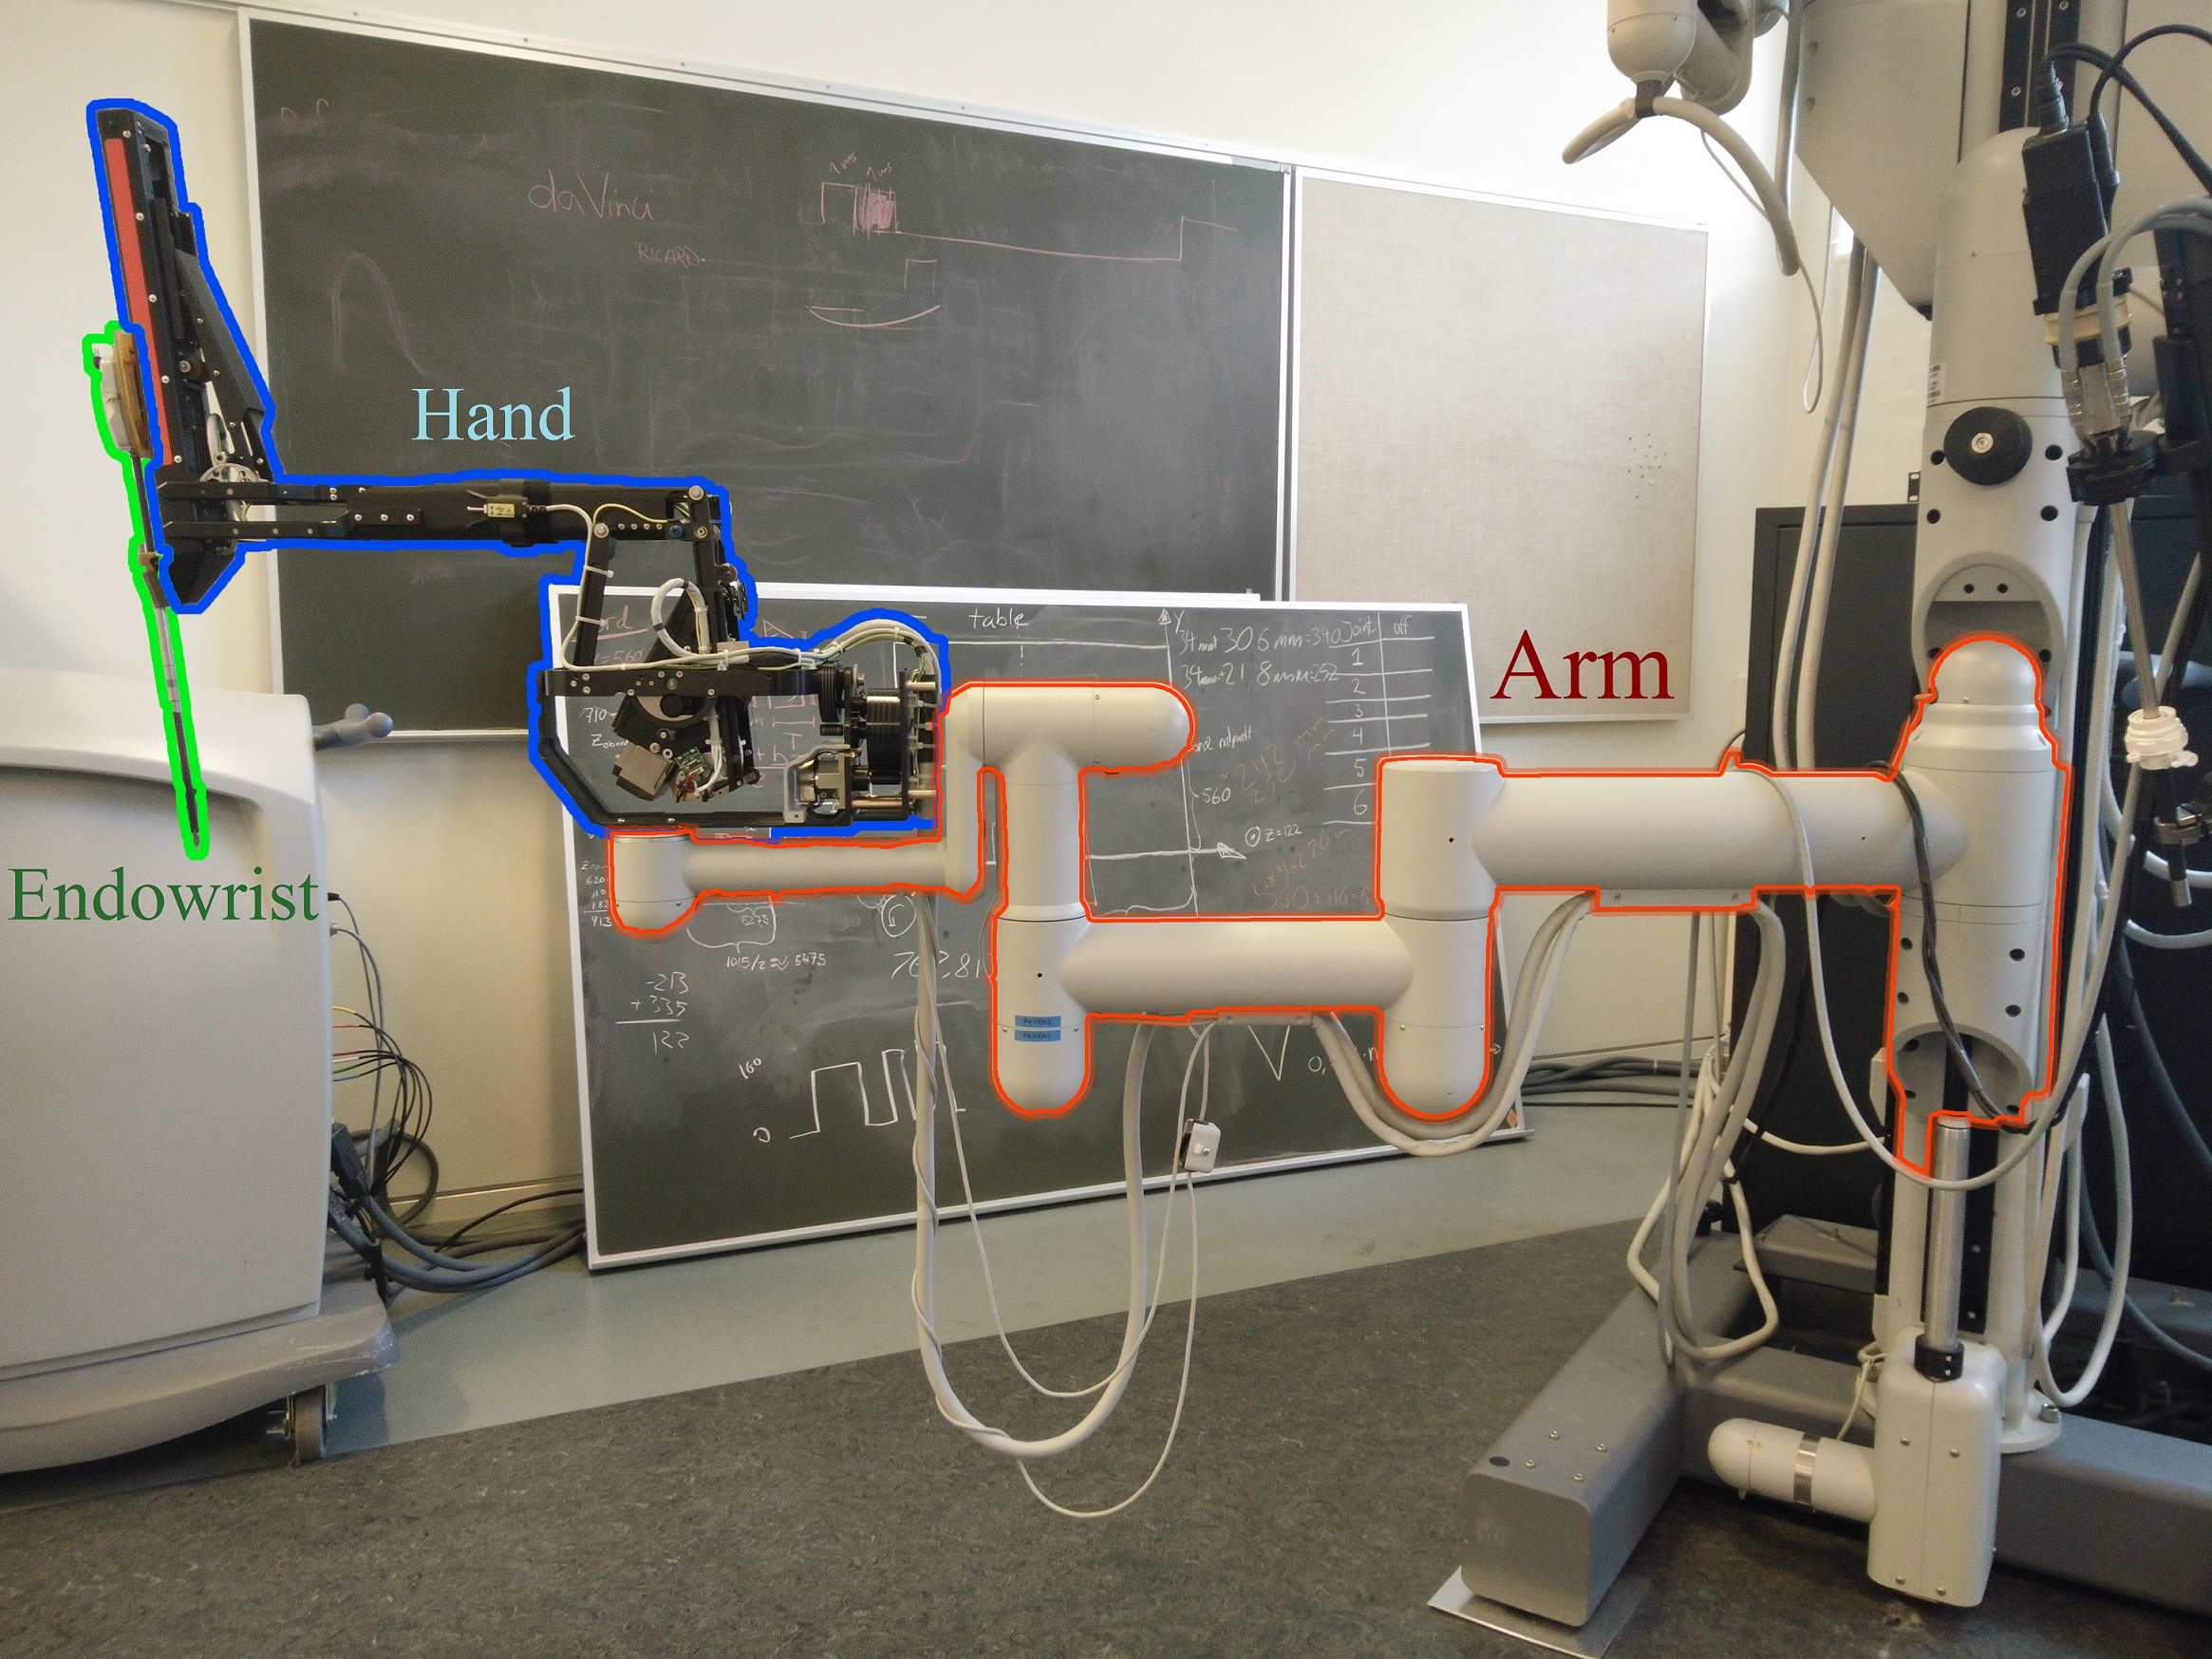
\includegraphics[width=0.85\linewidth]{davincirobotarm_label.jpg}
		\caption{One extended arm of the da vinci robot, where the arm, hand and tool are defined.}
		\label{fig:davinciarmrobot}
\end{figure}


\begin{enumerate}
\item Arm:

The arm of the tool is the part which is furtherest away from the patient. It is placed before the surgery and then locked in that position. Is is therefore not possible to alternate this position under surgery.
\item Hand

The hand is at the end of the arm and has three \gls{DOF}, which can be actuated under surgery.
\item Tool / end effector 

The tool is put together with the hand. Together these has 6 - 7 movable \gls{DOF}. The tool is the instrument which interacts with the patient under surgery. There are several different tools available, each with their own functionality. 
\end{enumerate}

